% CREATED BY WOLFGANG AHRENDT, 2021
% BASED ON A MASTER THESIS TEMPLATE CREATED BY DAVID FRISK, 2016,
%        MODIFIED BY JAKOB JARMAR 2016 AND GUSTAV ÖRTENBERG 2019

% COVER PAGE
\begin{titlepage}
\newgeometry{top=3cm, bottom=3cm,
			left=2.25 cm, right=2.25cm}	% Temporarily change margins		
			
% Cover page background 
\AddToShipoutPicture*{\backgroundpic{-4}{56.7}{figures/auxiliary/frontpage_gu_eng_vec_m2.pdf}}
\addtolength{\voffset}{2cm}

% Cover picture (replace with your own or delete)		
\begin{figure}[H]
\centering
%\vspace{0.5cm}	% Adjust vertical spacing here
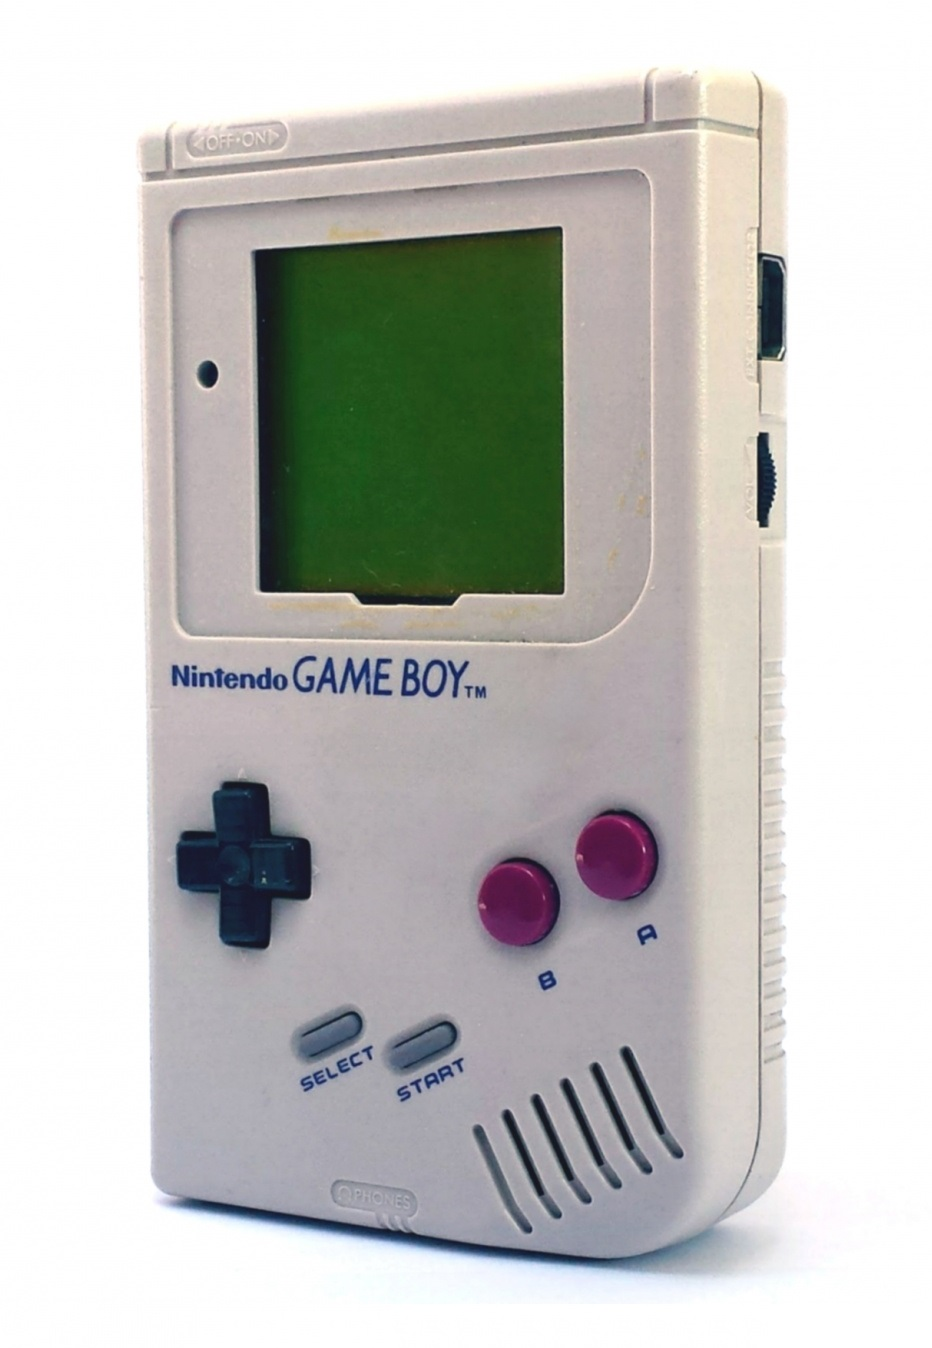
\includegraphics[scale=0.25]{figures/original-nintendo-gameboy2.jpg}
\end{figure}

% Cover text
\mbox{}
%\vfill
\renewcommand{\familydefault}{\sfdefault} \normalfont % Set cover page font

\textbf{\Huge \multiLineTitle{0.2cm}} 
\\[0.5cm]
%For subtitle uncomment below.
{\Large \oneLineSubtitle}\\[0.5cm]
%{\Large Emulating A Large System}\\[0.5cm]
Bachelor's thesis in Computer Science and Engineering

\setlength{\parskip}{1cm}

{\Large Algot Axelzon} \setlength{\parskip}{2.9cm}\\[1ex]
{\Large Isak Lindgren} \setlength{\parskip}{2.9cm}\\[1ex]
{\Large Carl Lindh} \setlength{\parskip}{2.9cm}\\[1ex]
{\Large David Möller} \setlength{\parskip}{2.9cm}\\[1ex]
{\Large Andreas Palmqvist} \setlength{\parskip}{2.9cm}\\[1ex]
{\Large Arvid Rydberg} \setlength{\parskip}{2.9cm}

Department of Computer Science and Engineering \\
\textsc{Chalmers University of Technology} \\
\textsc{University of Gothenburg} \\
Gothenburg, Sweden \the\year

\renewcommand{\familydefault}{\rmdefault} \normalfont % Reset standard font
\end{titlepage}


% BACK OF COVER PAGE (BLANK PAGE)
\newpage
\restoregeometry
\thispagestyle{empty}
\mbox{}

% TITLE PAGE
\newpage
\thispagestyle{empty}
\begin{center}
	\textsc{\large Bachelor's thesis \the\year}\\[4cm]		% Report number is currently not in use
	\textbf{\Large \multiLineTitle{0.2cm}} \\[1cm]

	{\large \oneLineSubtitle}\\[1cm]% Uncomment for subtitle
	{\large Algot Axelzon}\\[1ex]
	{\large Isak Lindgren}\\[1ex]
    {\large Carl Lindh}\\[1ex]
	{\large David Möller}\\[1ex]
	{\large Andreas Palmqvist}\\[1ex]
	{\large Arvid Rydberg}
	
	\vfill	
	% Logotype on titlepage	
	\begin{figure}[H]
	\centering
	% Remove the following line to remove the titlepage logotype
	
\includegraphics[width=0.25\pdfpagewidth]{figures/auxiliary/ChGULogoHog.pdf}
	\end{figure}	\vspace{5mm}	
	
	Department of Computer Science and Engineering\\
	%\emph{Division of Division name}\\
	%Name of research group (if applicable)\\
	\textsc{Chalmers University of Technology} \\
	\textsc{University of Gothenburg} \\
	Gothenburg, Sweden \the\year \\
\end{center}


% IMPRINT PAGE (BACK OF TITLE PAGE)
\newpage
\thispagestyle{plain}
%Place for rights to use?
\vspace*{4.5cm}
\oneLineTitle\\
\oneLineSubtitle\\ %Uncomment for subtitle
Algot Axelzon \setlength{\parskip}{1cm}
Isak Lindgren \setlength{\parskip}{1cm}
Carl Lindh \setlength{\parskip}{1cm}
David Möller \setlength{\parskip}{1cm}
Andreas Palmqvist \setlength{\parskip}{1cm}
Arvid Rydberg \setlength{\parskip}{1cm}

\copyright ~ Algot Axelzon, Isak Lindgren, Carl Lindh, David Möller, Andreas Palmqvist, Arvid Rydberg \the\year. \setlength{\parskip}{1cm}

Supervisor: Roc R. Currius, Department of Computer Science and Engineering\\
%(if applicable) Advisor: Name, Company or Institute\\
Examiner: Sven Knutsson, Department of Computer Science and Engineering \setlength{\parskip}{1cm}

Bachelor's Thesis \the\year\\	% Report number currently not in use 
Department of Computer Science and Engineering\\
%Division of Division name\\
%Name of research group (if applicable)\\
Chalmers University of Technology and University of Gothenburg\\
SE-412 96 Gothenburg\\
Telephone +46 31 772 1000 \setlength{\parskip}{0.5cm}

\vfill
% Caption for cover page figure if used, possibly with reference to further information in the report
Cover: Image of the original Game Boy from 1989. From \cite{OriginalGameBoy}. Public Domain.


%Typeset in \LaTeX \\
%Printed by [Name of printing company]\\
Gothenburg, Sweden \the\year

